% HISTORICAL ORIGIN
In this section we shortly introduce the principles of \textit{Hamiltonian Monte Carlo} or \textit{hybrid Monte Carlo} (HMC) that was originally introduced in \cite{MCMC:Duane1987}.
% INTRODUCTIONS
More comprehensive introductions can be found in \cite{MCMC:Liu2004,MCMC:Neal2011,MCMC:SanzSerna2014}.
% CORE IDEA
HMC sampling allows one to obtain a widely decorrelated posterior sample by suppressing the diffusive random walk behavior of standard MCMC techniques.
This is realized by embedding the parameter space in a higher-dimensional phase space and sampling from an appropriately defined auxiliary distribution that allows to extract the desired posterior as a marginal.
The formulation draws on the Hamiltonian formalism of classical mechanics.
More specifically it is inspired by a fictional classical particle moving in a potential well that is proportional to the negative log-density of the posterior.
Candidate states are proposed following a dynamical simulation in the augmented state space.
In doing so the search in the parameter space is guided by first-order derivative information from the posterior density.
It allows for nonlocal MCMC moves that span whole regions of the parameter space that carry significant posterior probability mass.
\par % HISTORY
HMC was originally developed for computational approaches to theoretical particle physics \cite{MCMC:Duane1987},
where it accelerates the stochastic simulation of high-dimensional integrals \cite{Physics:Gattringer2010}.
Afterwards the potential for statistical applications was recognized \cite{MCMC:Neal1996:a}.
% EXTENSIONS
Currently HMC has attracted greater attention in statistically and mathematically oriented scientific communities.
Numerous extensions and generalizations have been proposed in the recent literature \cite{MCMC:Shahbaba2014,MCMC:Papamarkou2014,MCMC:SohlDickstein2014,MCMC:Campos2015}.
% RIEMANNIAN MANIFOLD HMC
Notably there is the powerful yet costly Riemannian manifold HMC \cite{MCMC:Girolami2011,MCMC:Betancourt2013}.
% APPLICATION EXAMPLES
HMC and its enhanced variants are applied in an increasing number of studies \cite{MCMC:Beskos2013:b,MCMC:Elsheikh2014:a,MCMC:Kramer2014}.
\par % ENGINEERING EXAMPLES
However, HMC-like algorithms are still widely underacknowledged for engineering problems down to the present day.
Applications in structural dynamics and finite element modeling form exceptions \cite{MCMC:Cheung2009,MCMC:Boulkaibet2015}.
% HIERARCHICAL MODELS
Likewise this holds for hierarchical statistical models.
Although the software package Stan \cite{Computing:Stan2014} offers an adaptive HMC-variant \cite{MCMC:Hoffman2014} for classical hierarchical models, i.e.\ without physical forward modeling,
we are only aware of a very few studies wherein HMC is investigated \cite{MCMC:Zhang2014,MCMC:Betancourt2015}.
A semi-separable Hamiltonian for Riemannian manifold HMC sampling is proposed in \cite{MCMC:Zhang2014}.
Re-parametrizations of hierarchical models \cite{Multilevel:Papaspiliopoulos2007} in the context of HMC sampling are discussed in \cite{MCMC:Betancourt2015}.

\subsection{The MH algorithm}
% PRINCIPLE
The principle of MCMC sampling is the construction of an ergodic Markov chain over the prior support that has the posterior as its stationary distribution.
% METROPOLIS-HASTINGS
A prototypical class of MCMC techniques is based on the Metropolis-Hastings (MH) algorithm \cite{MCMC:Metropolis1953,MCMC:Hastings1970}.
% INTRODUCTIONS
More general introductions can be found in \cite{MCMC:Robert2004,MCMC:Brooks2011}.
\par % MCMC ITERATIONS
Let \(\pi_0(\bm{q})\) be the prior and \(\pi_1(\bm{q}) \propto \mathcal{L}(\bm{q}) \, \pi_0(\bm{q})\) the posterior of the unknown quantities \(\bm{q} = (q_1,\ldots,q_d) \in \mathds{R}^d\).
The MH algorithm is started at an initial state \(\bm{q}^{(0)}\) from the prior domain.
Then it realizes a Markov chain with a long-run distribution \(\pi_1(\bm{q})\) by repeatedly proceeding as follows.
For a state \(\bm{q}^{(t)}\) of the Markov chain in iteration \(t\), a candidate state \(\bm{q}^{(\star)} \sim P(\bm{q}^{(\star)} \cond \bm{q}^{(t)})\)
is sampled from an instrumental jumping distribution \(P(\bm{q}^{(\star)} \cond \bm{q}^{(t)})\).
This proposal is then accepted as the new state with probability
\begin{equation} \label{eq:MCMC:MHCorrection}
  \alpha \left( \bm{q}^{(\star)} \cond \bm{q}^{(t)} \right)
  \, = \, \operatorname{min} \left\{ 1,\frac{\pi_1(\bm{q}^{(\star)}) \, P(\bm{q}^{(t)} \cond \bm{q}^{(\star)})}{\pi_1(\bm{q}^{(t)}) \, P(\bm{q}^{(\star)} \cond \bm{q}^{(t)})} \right\}.
\end{equation}
In this case the new state in iteration \(t+1\) is \(\bm{q}^{(t+1)} = \bm{q}^{(\star)}\).
In case of rejection the chain remains in its state \(\bm{q}^{(t+1)} = \bm{q}^{(t)}\).
% DETAILED BALANCE
The Markov chain transition kernel defined this way is easily seen to satisfy detailed balance with respect to the posterior.
This is a sufficient condition for leaving the posterior invariant.
% UNSCALED POSTERIOR
An appealing feature of the MH correction \cref{eq:MCMC:MHCorrection} is that it only calls for evaluations of the unscaled posterior density.
% PROPOSAL DISTRIBUTION
Moreover it gives ample scope for the design of efficient proposal distributions \(P\).
\par % RANDOM WALK SAMPLING
A common MCMC updating scheme is the random walk Metropolis (RWM) sampler.
It is based on local proposals that are sampled from a Gaussian distribution \(\mathcal{N}(\bm{q}^{(\star)} \cond \bm{q}^{(t)},\bm{\Sigma}_{\bm{q}})\) with mean \(\bm{q}^{(t)}\) and covariance matrix \(\bm{\Sigma}_{\bm{q}}\).
This leads to the classical diffusive random walk behavior.
Note that for this symmetric proposals the acceptance probability in \cref{eq:MCMC:MHCorrection} reduces to \(\alpha = \operatorname{min} \{ 1,\pi_1(\bm{q}^{(\star)}) / \pi_1(\bm{q}^{(t)}) \}\).
% OPTIMAL SCALING
Optimal scalings of the RWM in high-dimension are investigated in \cite{MCMC:Roberts1997:b,MCMC:Roberts2001}.

\subsection{Effective sample size}
% AUTOCORRELATION
Due to the Markovian updates MCMC samples are generally autocorrelated.
The autocorrelation governs the quality of the MCMC sample with respect to posterior expectations \(\mu_g = \mathds{E}[g(\bm{q})] = \int g(\bm{q}) \pi_1(\bm{q}) \, \mathrm{d} \bm{q}\)
of a function of interest \(g \colon \mathds{R}^d \rightarrow \mathds{R}\) \cite{MCMC:Geyer1992,MCMC:Tierney1994}.
% CENTRAL LIMIT THEOREM
Under certain conditions one can show that the Markov chain \(\bm{q}^{(0)},\bm{q}^{(1)},\bm{q}^{(2)},\ldots\) satisfies a central limit theorem \cite{MCMC:Jones2004,MCMC:Roberts2004}.
For a large number of iterations \(N \rightarrow \infty\) the sample means \(\bar{g} = N^{-1} \sum_{t=1}^N g_t\) with \(g_t = g(\bm{q}^{(t)})\)
approach a Gaussian distribution \(\mathcal{N}(\bar{g} \cond \mu_{\bar{g}},\sigma^2_{\bar{g}})\) with mean \(\mu_{\bar{g}} = \mu_g\) and asymptotic variance
\begin{equation} \label{eq:MCMC:EstimationVariance}
  \sigma^2_{\bar{g}} = \frac{\sigma^2_{g}}{N} \left( 1 + 2 \sum\limits_{s=1}^{\infty} \rho_s \right) = \frac{\sigma^2_{g}}{N} \tau_{\mathrm{int}} = \frac{\sigma^2_{g}}{N_{\mathrm{eff}}}.
\end{equation}
Here the variance \(\sigma^2_{g} = \mathrm{Var}[g_t]\) and the lag-\(s\) autocorrelation \(\rho_s = \mathrm{Cov}[g_t,g_{t+s}] / \sigma^2_{g}\) are statistical moments with respect to the stationary distribution.
% EFFECTIVE SAMPLE SIZE
The \textit{integrated autocorrelation time} in \cref{eq:MCMC:EstimationVariance} is defined as \(\tau_{\mathrm{int}} = 1 + 2 \sum_{s=1}^{\infty} \rho_s\).
Based on this one can define an \textit{effective sample size} \(N_{\mathrm{eff}} = N / \tau_{\mathrm{int}}\)
which quantifies an equivalent number of independent draws from the posterior featuring the same standard error \(\sigma_{\bar{g}} = \sigma_{g} / \sqrt{N_{\mathrm{eff}}}\) as the autocorrelated MCMC sample of size \(N\).
In this sense \(\tau_{\mathrm{int}}\) and \(N_{\mathrm{eff}}\) are measures of the imprecision and effectiveness of simulating \(\mu_g\) as \(\bar{g}\), respectively.
% STATISITICAL PARAMETERS
Note that with the projection \(g \colon \bm{q} \mapsto q_j\) for \(j \in \{1,\ldots,d\}\) these considerations straightforwardly apply to each posterior marginal.

\subsection{Systems from classical physics}
% ANALOGIES
By analogy with two systems from classical physics, i.e.\ Newtonian and statistical mechanics \cite{Physics:Deriglazov2010,Physics:Schwabl2006}, the basic machinery of HMC is now outlined.
% HAMILTONIAN
We consider a hypothetical classical system with \textit{canonical coordinates} \((\bm{q},\bm{p})\), i.e.\ the \textit{positions} \(\bm{q} \in \mathds{R}^d\) and \textit{conjugate momenta} \(\bm{p} \in \mathds{R}^d\).
Statistical QoI \(\bm{q}\) are identified with positions of the system and momentum variables \(\bm{p}\) are additionally introduced.
The \textit{Hamiltonian} of the system is given as
\begin{equation} \label{eq:HMC:Hamiltonian}
  H(\bm{q},\bm{p}) = V(\bm{q}) + T(\bm{p}),
\end{equation}
where \(V(\bm{q})\) and \(T(\bm{p})\) are the \textit{potential} and \textit{kinetic energy}, respectively.
% POTENTIAL ENERGY
The potential energy in \cref{eq:HMC:Hamiltonian} is defined as
\begin{equation} \label{eq:HMC:PotentialEnergy}
  V(\bm{q}) = - \log \left( \mathcal{L}(\bm{q}) \, \pi_0(\bm{q}) \right),
\end{equation}
where \(\pi_0(\bm{q})\) and \(\mathcal{L}(\bm{q})\) are the prior density and the likelihood function, respectively.
% KINETIC ENERGY
The kinetic energy term in \cref{eq:HMC:Hamiltonian} is defined as
\begin{equation} \label{eq:HMC:KineticEnergy}
  T(\bm{p}) = \frac{\bm{p}^{\top} \bm{M}^{-1} \bm{p}}{2},
\end{equation}
where \(\bm{M}\) is some symmetric and positive-definite \textit{mass matrix}.
Often it is a multiple \(\bm{M} = m \bm{I}_d\) of the identity matrix \(\bm{I}_d\) or of the general diagonal form \(\bm{M} = \operatorname{diag}(m_1,\ldots,m_d)\).
\par % ANALOGY: HAMILTONIAN DYNAMICS
As a first analogy to classical physics one considers \textit{Hamiltonian dynamics} \cite{Physics:Deriglazov2010}.
% EQUATION OF MOTION
The evolution of the system in fictitious time \(\tau\) is then governed by Hamilton's equations of motion (EoM)
\begin{equation} \label{eq:HMC:EOM}
  \frac{\mathrm{d} \bm{q}}{\mathrm{d} \tau} =   \frac{\partial H}{\partial \bm{p}}, \quad
  \frac{\mathrm{d} \bm{p}}{\mathrm{d} \tau} = - \frac{\partial H}{\partial \bm{q}}.
\end{equation}
% DETERMINISTIC MAP
The governing differential equations in \cref{eq:HMC:EOM} determine the system trajectory over time.
% DYNAMICAL PROPERTIES 
This dynamics satisfies time reversibility (invariance of the dynamics under the transformation \((\tau,\bm{p}) \mapsto (-\tau,-\bm{p})\)),
energy conservation (\(\mathrm{d} H / \mathrm{d} \tau = 0\)) and preservation of the phase space volume (Liouville's theorem).
\par % ANALOGY: CANONICAL ENSEMBLE
As a second analogy to classical physics one considers the distribution of the \textit{canonical ensemble} from statistical mechanics \cite{Physics:Schwabl2006}.
The fictitious temperature and the Boltzmann constant are set to one.
% CANONICAL JOINT DISTRIBUTION
Then the frequency distribution of the positions and the momenta is the \textit{Boltzmann distribution}
\begin{equation} \label{eq:HMC:BoltzmannDistribution}
  \varPi_1(\bm{q},\bm{p}) = \frac{1}{Z} \exp (-H(\bm{q},\bm{p})) = \frac{\mathcal{L}(\bm{q}) \, \pi_0(\bm{q})}{Z} \, \exp \left( - \frac{\bm{p}^{\top} \bm{M}^{-1} \bm{p}}{2} \right).
\end{equation}
Here the normalizing constant \(Z\) is the \textit{canonical partition function}.
It does not have to be explicitly known for HMC sampling.
By construction, i.e.\ due to the definitions in \cref{eq:HMC:Hamiltonian,eq:HMC:KineticEnergy,eq:HMC:PotentialEnergy},
the joint distribution \cref{eq:HMC:BoltzmannDistribution} has the form \(\varPi_1(\bm{q},\bm{p}) = \pi_1(\bm{q}) \, \pi_1(\bm{p})\). 
% POSTERIOR AS MARGINAL
It features the posterior \(\pi_1(\bm{q}) \propto \exp(-V(\bm{q})) = \mathcal{L}(\bm{q}) \, \pi_0(\bm{q})\) as its \(\bm{q}\)-marginal.
% GAUSSIAN MARGINAL
Moreover the \(\bm{p}\)-marginal of \cref{eq:HMC:BoltzmannDistribution} is a multivariate Gaussian \(\pi_1(\bm{p}) \propto \exp(-T(\bm{p})) = \exp (\bm{p}^{\top} \bm{M}^{-1} \bm{p} / 2)\) with covariance matrix \(\bm{M}\).
The partition function \(Z\) absorbs the normalization factors of \(\pi_1(\bm{q})\) and \(\pi_1(\bm{p})\).

\subsection{The HMC algorithm}
% CORE IDEA
The core idea of HMC is to realize an ergodic Markov chain over the \(2d\)-dimensional configuration space of the classical system that was defined above.
This chain is constructed in such a way that it features \cref{eq:HMC:BoltzmannDistribution} as its stationary distribution, with the posterior as a marginal.
% MARKOVIAN TRANSITIONS
After the HMC algorithm is initialized at a certain \(\bm{q}^{(0)}\) one iteratively applies the following Markovian transition.
Given the current positions \(\bm{q}^{(t)}\) of the Markov chain at iteration \(t\),
the corresponding momenta are directly sampled from the distribution \(\pi_1(\bm{p}^{(t)}) = \mathcal{N}(\bm{p}^{(t)} \cond \bm{0},\bm{M})\).
The system configuration \((\bm{q}^{(t)},\bm{p}^{(t)})\) is then evolved over some arbitrary time interval, after which it has reached a new configuration \((\bm{q}^{(\star)},\bm{p}^{(\star)})\).
Following this, the updated position \(\bm{q}^{(\star)}\) is the new state \(\bm{q}^{(t+1)}\) of the Markov chain in iteration \(t+1\), i.e.\ acceptance by default.
Since we are only interested in positions, the auxiliary momentum \(\bm{p}^{(\star)}\) is discarded.
% INVARIANT DISTRIBUTION
Time reversibility, the conservation of energy and the preservation phase space volume are important dynamical properties of the EoM in \cref{eq:HMC:EOM}.
Based on the latter two properties one can show that the transition defined above leaves the Boltzmann distribution \cref{eq:HMC:BoltzmannDistribution} invariant \cite{MCMC:SanzSerna2014}.
\par % ADVANTAGES
The abovementioned ideal HMC updating scheme avoids the symmetric and strongly localized proposals of RWM-type algorithms.
Properly tuned the dynamical transitions may cover wide regions of the position space that accumulate significant posterior mass.
It can be extremely efficient for sampling high-dimensional and strongly correlated posterior distributions.
% HIERARCHICAL MODELS
This makes HMC a promising candidate sampler for hierarchical models that are higher-dimensional and correlated per definition.
\par % LEAPFROG SCHEME
In practice idealized HMC updating based on exactly solving the EoM cannot be accomplished.
Instead one has to resort to numerical simulations of Hamiltonian dynamics based on suitable integrators \cite{Physics:Sanz-Serna1994,Physics:Leimkuhler2004}.
A standard choice is the \textit{leapfrog} time-stepping scheme \cite{Physics:Hairer2003}, but note that also other symplectic integrators could be used \cite{MCMC:Blanes2014}.
The system is evolved from its configuration at time \(\tau_1\) into the one at \(\tau_2 > \tau_1\) by an iterative computation of the position and momentum variables
\begin{subequations} \label{eq:HMC:LeapfrogScheme}
  \begin{align}
    \bm{q}(\tau + \Delta\tau) &= \bm{q}(\tau) + \Delta\tau \bm{M}^{-1} \bm{p} (\tau + \frac{1}{2} \Delta\tau), \label{eq:HMC:LeapfrogScheme:q} \\
    \bm{p}(\tau + \frac{3}{2} \Delta\tau) &= \bm{p}(\tau + \frac{1}{2} \Delta\tau) - \Delta\tau \frac{\partial V}{\partial \bm{q}} (\bm{q}(\tau + \Delta\tau)) \label{eq:HMC:LeapfrogScheme:p}.
  \end{align}
\end{subequations}
Starting from \((\bm{q}(\tau_1),\bm{p}(\tau_1)) \equiv (\bm{q}^{(t)},\bm{p}^{(t)})\) the momentum
\(\bm{p}(\tau_1 + \frac{1}{2} \Delta\tau) = \bm{p}(\tau_1) - \frac{1}{2} \Delta\tau \frac{\partial V}{\partial \bm{q}} (\bm{q}(\tau_1))\) is computed in a half step.
Thereafter alternating full steps are done for the positions and momenta according to \cref{eq:HMC:LeapfrogScheme}.
Finally a half step is taken from \(\bm{p}(\tau_2 - \frac{1}{2} \Delta\tau)\) to
\(\bm{p}(\tau_2) = \bm{p}(\tau_2 - \frac{1}{2} \Delta\tau) - \frac{1}{2} \Delta\tau \frac{\partial V}{\partial \bm{q}} (\bm{q}(\tau_2))\).
At the end the system has evolved into \((\bm{q}(\tau_2),\bm{p}(\tau_2)) \equiv (\bm{q}^{(\star)},\bm{p}^{(\star)})\).
% DISCRETIZATION
This way the computation over the time interval \(\tau_2 - \tau_1 = L \Delta\tau\) has been discretized into a discrete number of steps \(L\) with a finite stepsize \(\Delta\tau\).
% VISUALIZATION
A visualization of this time integration scheme is provided in \cref{fig:Leapfrog}.
The full and half steps of the time evolution of the system are shown.
\begin{figure}[ht]
  \centering
  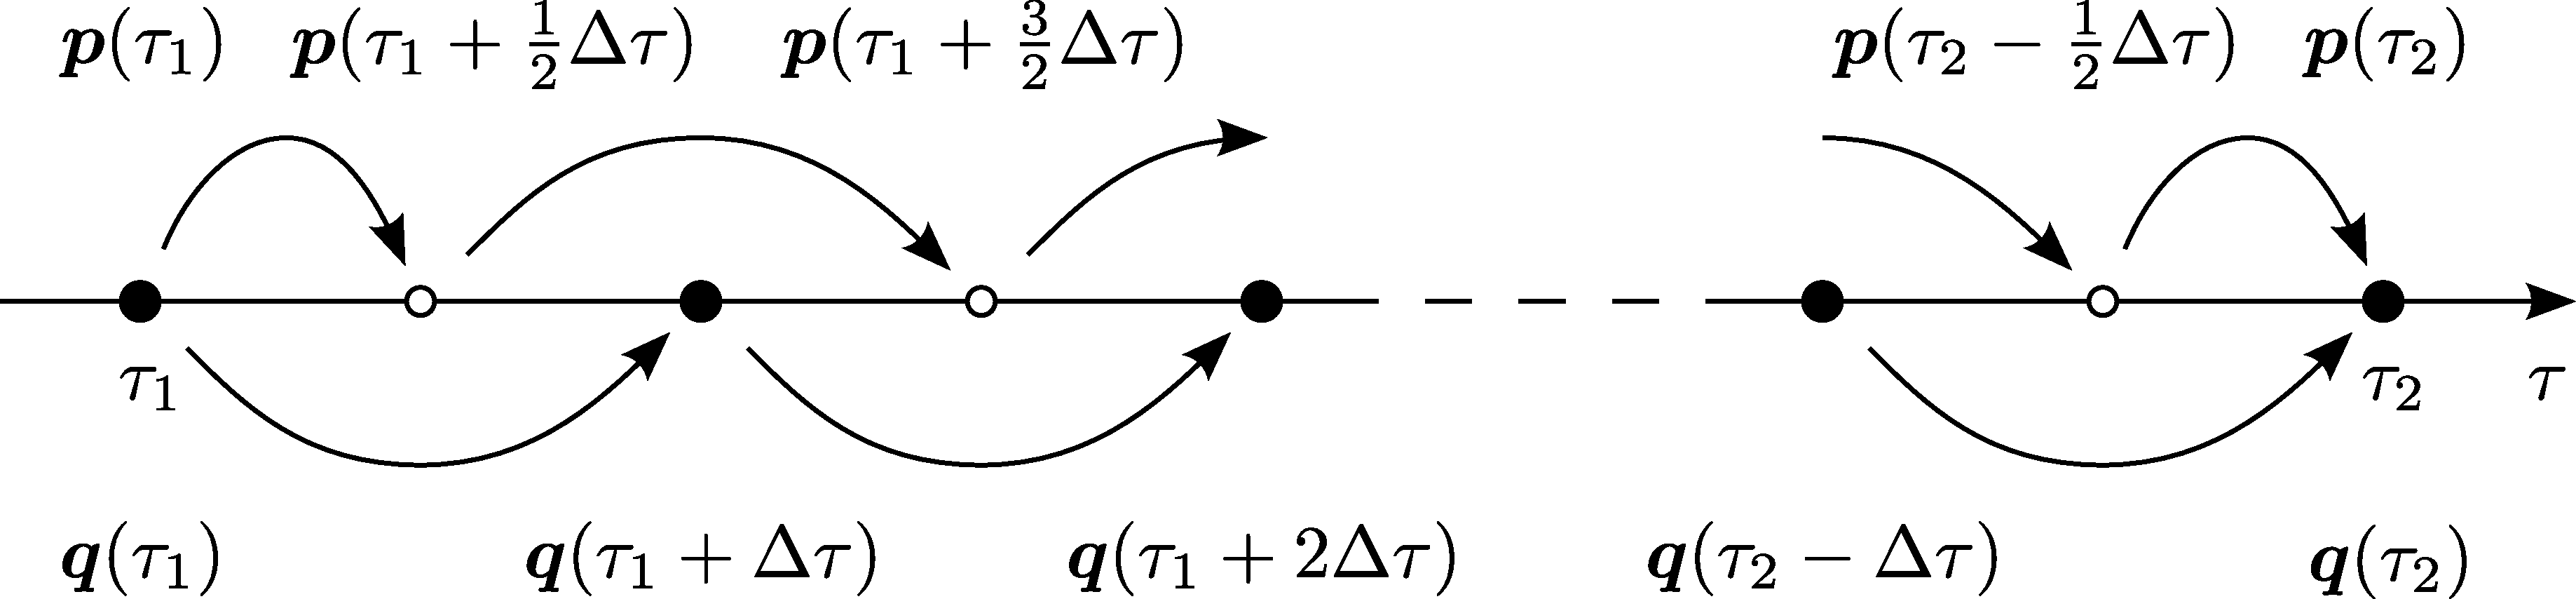
\includegraphics[width=\JRUESleapWidth]{fig_JRUES_Leapfrog}
  \caption[Leapfrog time stepping]{Leapfrog time stepping.}
  \label{fig:Leapfrog}
\end{figure}
\par % PROPERTIES OF THE LEAPFROG
An appealing property of the leapfrog is that it approximates Hamiltonian dynamics in a way that exactly maintains time reversibility and volume preservation.
The total energy is approximately conserved with an error that asymptotically is of the order \(\mathcal{O}(\Delta\tau^2)\).
This introduces a characteristic scale of the stepsize that is related to stable trajectories.
% MH ACCEPTANCE
In order to compensate for the introduced approximation of Hamiltonian dynamics, candidate configurations \((\bm{q}^{(\star)},\bm{p}^{(\star)})\) are accepted with probability
\begin{equation} \label{eq:HMC:MHCorrection}
  \alpha \left( \bm{p}^{(\star)}, \bm{q}^{(\star)} \cond \bm{p}^{(t)}, \bm{q}^{(t)} \right)
  \, = \, \operatorname{min} \left\{ 1,  \exp \left( H \left( \bm{p}^{(t)},\bm{q}^{(t)} \right) - H \left( \bm{p}^{(\star)},\bm{q}^{(\star)} \right) \right) \right\}.
\end{equation}
% SYMMETRIC PROPOSAL
This is plain vanilla Metropolis correction in the \(2d\)-dimensional phase space for a symmetric proposal distribution \cite{MCMC:SanzSerna2014}.
Volume preservation and time reversibility of the leapfrog integration are the properties that ensure the symmetry in the proposals.
Strictly speaking one would have to negate the momenta at the end of the trajectory, however, those are disregarded anyhow.
Due to \cref{eq:HMC:MHCorrection} the acceptance rate depends on the degree as to which energy conservation is violated.
% DETAILED BALANCE
The combined transition satisfies detailed balance with respect to the Boltzmann distribution \cref{eq:HMC:BoltzmannDistribution}.
Thus the Markov chain \(\bm{q}^{(0)},\bm{q}^{(1)},\bm{q}^{(2)},\ldots\) exhibits the stationary distribution \(\pi_1(\bm{q})\).
% POSTERIOR RATIOS
Notice that, similar to the MH algorithm, HMC sampling requires only evaluations of the unnormalized posterior density.
\par % PARTIAL DERIVATIVES
Additionally the time integration in \cref{eq:HMC:LeapfrogScheme} requires the computation of first-order partial derivatives of the unscaled posterior log-density in \cref{eq:HMC:PotentialEnergy}.
In turn this requires the differentiation of the forward model with respect to its inputs.
For simple models this can be done analytically \cite{Nagel:ICVRAM2014:Proc}.
Otherwise one has to rely on the adjoint method \cite{MCMC:BuiThanh2014}, automatic differentiation \cite{MCMC:Cheung2009} or the straightforward use of finite differences \cite{MCMC:Boulkaibet2015}.
It is interesting to note that derivatives do not have to be calculated exactly.
Although this may decrease the acceptance rate, such approximations are managed in the correction step \cref{eq:HMC:MHCorrection}.
% PCE-DRIVEN PCE
An interesting idea would be to employ such approximations of the forward model for which derivatives can be analytically obtained, e.g.\ polynomial chaos metamodels \cite{PCE:Sudret2015}.
\par % INPUT CONSTRAINTS
Other practical issues relate to the handling of parameter constraints \cite{MCMC:Pakman2014,MCMC:Lan2014} and the optimal tuning of the algorithm \cite{MCMC:Beskos2013:a,MCMC:Betancourt2014:arXiv}.
% ADJUSTABLE PARAMETERS
Free algorithmic parameters of the HMC are the number of leapfrog steps \(L\) and the timestep \(\Delta\tau\).
Together they determine the total trajectory length \(L \Delta\tau\).
Furthermore the mass matrix \(\bm{M}\) has to be set.
The latter is often chosen to be a diagonal matrix \(\bm{M} = \operatorname{diag}(m_1,\ldots,m_d)\).
Individually setting the entries \(m_i\) for \(i=1,\ldots,d\) then allows to account for different posterior scales of \(q_i\),
e.g.\ with \(m_i = 1/\mathrm{Var}[q_i]\) where \(\mathrm{Var}[q_i]\) is the marginal posterior variance.
A more in-depth discussion of related issues is found in \cite{MCMC:Neal2011}.